\documentclass{ieeeaccess}

\usepackage{cite}
\usepackage{amsmath,amsfonts}
\usepackage{algorithmic}
\usepackage{graphicx}
\usepackage{textcomp}

\usepackage{url}
\usepackage{breakurl}
\def\UrlBreaks{\do\/\do-} %hack to force url breaks on "-" in references

\usepackage[colorlinks,
	linkcolor={[rgb]{0,0,0.4}},
	urlcolor ={[rgb]{0,0,1}}, 
	citecolor={[rgb]{0,0,0.4}},
	]{hyperref}

\usepackage{hyperref}
\renewcommand{\sectionautorefname}{\S}
\renewcommand{\subsectionautorefname}{\S}
\renewcommand{\subsubsectionautorefname}{\S}

\usepackage{color}
\usepackage{caption}
\usepackage{subcaption}
\usepackage{threeparttable}
\usepackage{multirow}
\usepackage{booktabs}
\usepackage{verbatim}
\usepackage{epstopdf}
\usepackage{rotating}
\usepackage{listings}
\usepackage{listing}
\usepackage{paralist}
\usepackage{arydshln}
\let\labelindent\relax
\usepackage{enumitem}
\usepackage{amssymb}
\usepackage{balance}
\usepackage{endnotes}
\usepackage{xspace}
\usepackage{times}
\usepackage{pifont}
\usepackage{wasysym}
% \usepackage{tikz}
% \usepackage{algpseudocode}% http://ctan.org/pkg/algorithmicx
\usepackage[ruled,vlined,linesnumbered]{algorithm2e}

\def\BibTeX{{\rm B\kern-.05em{\sc i\kern-.025em b}\kern-.08em
    T\kern-.1667em\lower.7ex\hbox{E}\kern-.125emX}}


\newcommand{\Tstrut}{\rule{0pt}{2.6ex}}         % = `top' strut
\newcommand{\Bstrut}{\rule[-0.9ex]{0pt}{0pt}}   % = `bottom' strut

% \newcommand{\commentontext}[2]{\colorbox{yellow}{#1}\pdfcomment[color={0.234 0.867 0.211},hoffset=-6pt,voffset=10pt,opacity=0.5]{#2}}
% \newcommand{\commentatside}[1]{\pdfcomment[color={0.045 0.278 0.643},icon=Note]{#1}}
% Compatibality with packages todo, easy-todo, todonotes
% \newcommand{\todo}[1]{\commentatside{#1}}
% Compatiblity with package fixmetodonotes
% \newcommand{\TODO}[1]{\commentatside{#1}}

\newcommand{\etc}{\textit{etc.}}
\newcommand{\ie}{\textit{i.e.}}
\newcommand{\tick}{\ding{51}}
\newcommand{\cross}{\ding{55}}

\graphicspath{{./figs/}}


\begin{document}
\history{Date of publication xxxx 00, 0000, date of current version xxxx 00, 0000.}
\doi{10.1109/ACCESS.2017.DOI}

\title{Preparation of Papers for IEEE ACCESS}
\author{\uppercase{First A. Author}\authorrefmark{1}, \IEEEmembership{Fellow, IEEE},
\uppercase{Second B. Author\authorrefmark{2}, and Third C. Author,
Jr}.\authorrefmark{3},
\IEEEmembership{Member, IEEE}}
\address[1]{National Institute of Standards and 
Technology, Boulder, CO 80305 USA (e-mail: author@boulder.nist.gov)}
\address[2]{Department of Physics, Colorado State University, Fort Collins, 
CO 80523 USA (e-mail: author@lamar.colostate.edu)}
\address[3]{Electrical Engineering Department, University of Colorado, Boulder, CO 
80309 USA}
\tfootnote{This paragraph of the first footnote will contain support 
information, including sponsor and financial support acknowledgment. For 
example, ``This work was supported in part by the U.S. Department of 
Commerce under Grant BS123456.''}

\markboth
{Author \headeretal: Preparation of Papers for IEEE TRANSACTIONS and JOURNALS}
{Author \headeretal: Preparation of Papers for IEEE TRANSACTIONS and JOURNALS}

\corresp{Corresponding author: First A. Author (e-mail: author@ boulder.nist.gov).}


\begin{abstract}
	\begin{abstract}
abstract
\end{abstract}

\end{abstract}


\begin{keywords}
Enter key words or phrases in alphabetical 
order, separated by commas. For a list of suggested keywords, send a blank 
e-mail to keywords@ieee.org or visit \underline
{http://www.ieee.org/organizations/pubs/ani\_prod/keywrd98.txt}
\end{keywords}

\titlepgskip=-15pt

\maketitle


\section{Introduction}
\label{s:intro}

\begin{figure}[h]
	\centering
	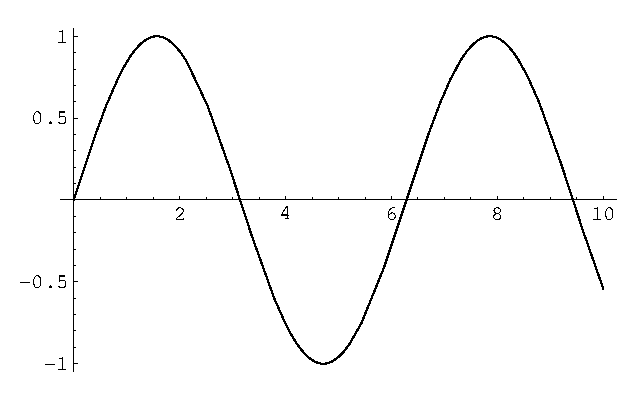
\includegraphics[width=0.8\linewidth]{sample}
	\caption{Sample}
	\label{f:sample}
\end{figure}

see this~\cite{latex}
\section{Background}
\label{s:backg}

\section{Design}
\label{s:design}

\section{Implementation}
\label{s:impl}

\section{Evaluation}
\label{s:eval}

\section{Related work}
\label{s:relwk}
\section{Conclusion}
\label{s:conclusion}

\section{Acknowledgment}
\label{s:ack}



\bibliographystyle{abbrv}
\bibliography{references}

\appendices
\section{Appendix}

This should be Appendix A!


\begin{IEEEbiography}[{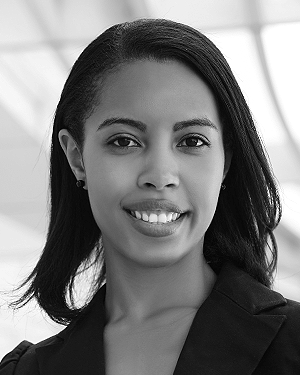
\includegraphics[width=1in,height=1.25in,clip,keepaspectratio]{a1.png}}]{First A. Author} (M'76--SM'81--F'87) and all authors may include 
biographies. Biographies are often not included in conference-related
papers. This author became a Member (M) of IEEE in 1976, a Senior
Member (SM) in 1981, and a Fellow (F) in 1987. The first paragraph may
contain a place and/or date of birth (list place, then date). Next,
the author's educational background is listed. The degrees should be
listed with type of degree in what field, which institution, city,
state, and country, and year the degree was earned. The author's major
field of study should be lower-cased. 

The second paragraph uses the pronoun of the person (he or she) and not the 
author's last name. It lists military and work experience, including summer 
and fellowship jobs. Job titles are capitalized. The current job must have a 
location; previous positions may be listed 
without one. Information concerning previous publications may be included. 
Try not to list more than three books or published articles. The format for 
listing publishers of a book within the biography is: title of book 
(publisher name, year) similar to a reference. Current and previous research 
interests end the paragraph. The third paragraph begins with the author's 
title and last name (e.g., Dr.\ Smith, Prof.\ Jones, Mr.\ Kajor, Ms.\ Hunter). 
List any memberships in professional societies other than the IEEE. Finally, 
list any awards and work for IEEE committees and publications. If a 
photograph is provided, it should be of good quality, and 
professional-looking. Following are two examples of an author's biography.
\end{IEEEbiography}

\begin{IEEEbiography}[{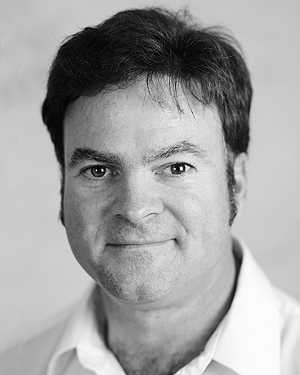
\includegraphics[width=1in,height=1.25in,clip,keepaspectratio]{a2.png}}]{Second B. Author} was born in Greenwich Village, New York, NY, USA in 
1977. He received the B.S. and M.S. degrees in aerospace engineering from 
the University of Virginia, Charlottesville, in 2001 and the Ph.D. degree in 
mechanical engineering from Drexel University, Philadelphia, PA, in 2008.

From 2001 to 2004, he was a Research Assistant with the Princeton Plasma 
Physics Laboratory. Since 2009, he has been an Assistant Professor with the 
Mechanical Engineering Department, Texas A{\&}M University, College Station. 
He is the author of three books, more than 150 articles, and more than 70 
inventions. His research interests include high-pressure and high-density 
nonthermal plasma discharge processes and applications, microscale plasma 
discharges, discharges in liquids, spectroscopic diagnostics, plasma 
propulsion, and innovation plasma applications. He is an Associate Editor of 
the journal \emph{Earth, Moon, Planets}, and holds two patents. 

Dr. Author was a recipient of the International Association of Geomagnetism 
and Aeronomy Young Scientist Award for Excellence in 2008, and the IEEE 
Electromagnetic Compatibility Society Best Symposium Paper Award in 2011. 
\end{IEEEbiography}

\begin{IEEEbiography}[{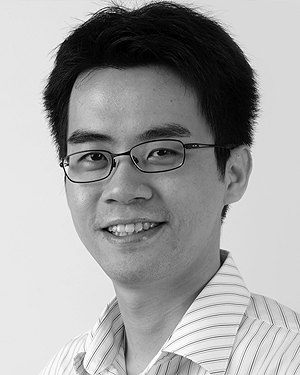
\includegraphics[width=1in,height=1.25in,clip,keepaspectratio]{a3.png}}]{Third C. Author, Jr.} (M'87) received the B.S. degree in mechanical 
engineering from National Chung Cheng University, Chiayi, Taiwan, in 2004 
and the M.S. degree in mechanical engineering from National Tsing Hua 
University, Hsinchu, Taiwan, in 2006. He is currently pursuing the Ph.D. 
degree in mechanical engineering at Texas A{\&}M University, College 
Station, TX, USA.

From 2008 to 2009, he was a Research Assistant with the Institute of 
Physics, Academia Sinica, Tapei, Taiwan. His research interest includes the 
development of surface processing and biological/medical treatment 
techniques using nonthermal atmospheric pressure plasmas, fundamental study 
of plasma sources, and fabrication of micro- or nanostructured surfaces. 

Mr. Author's awards and honors include the Frew Fellowship (Australian 
Academy of Science), the I. I. Rabi Prize (APS), the European Frequency and 
Time Forum Award, the Carl Zeiss Research Award, the William F. Meggers 
Award and the Adolph Lomb Medal (OSA).
\end{IEEEbiography}

\EOD


\end{document}
